\section{Server Provisioning Policies}
\label{sec:provision}
\vspace*{\subsecspace}

Resource provisioning, i.e., determining the size and capacity of the servers for handling FaaS workloads, is a fundamental problem in serverless computing. 
In this section, we develop techniques that allocate the appropriate amount of resources to servers based on the characteristics of the function workloads. 
Resource provisioning policies must consider the rate of function invocations, the resource footprints of the functions, and the inter-arrival time between function invocations. 
To handle the interplay and tradeoffs between these factors, we use similar principles for provisioning that we used for developing our keep-alive policies. 
% Previous three lines are a bit verbose and can be compressed to 2, but ok.. 

The fundamental challenge underlying resource provisioning for FaaS workloads is the performance vs. resource allocation tradeoff. 
Running a workload on large servers/VMs provides more resources for the keep-alive cache, which reduces the cold starts and improves the application performance. 
However, we must also be careful to not \emph{overprovision}, since it leads to wasted and underutilized resources.
Additionally, since function workload can be dynamic, resource provisioning must be \emph{elastic}, and be able to dynamically scale up or down based on the load. 
We therefore present a \emph{static} provisioning policy that determines the server memory size for a given function workload, and then develop an elastic-scaling approach for handling workload temporal dynamics. 

\subsection{Static Provisioning}
\label{subsec:static}
\vspace*{\subsecspace}

In the last section, we have seen how keeping function containers warm in a keep-alive cache can help mitigate the cold start overheads. 
The effectiveness of any keep-alive policy depends on the size of this keep-alive cache, and thus the server resources available, i.e., the server size. 
Our \emph{static} provisioning policy thus selects a server size for handling a given workload. 
% Not peak, since that would be infinite sized. 90 percentile, but we dont do that. 
We want to optimize the resource provisioning to avoid over and under provisioning, both of which are detrimental to cost and performance respectively. 


Having established that keep-alive policies are equivalent to cache eviction in the previous section, we now extend the use of the caching analogy further, to develop a caching-based provisioning approach. 
We claim that the performance vs. resource availability tradeoff of serverless functions can be understood and modeled using cache hit (or miss) ratio curves.
%
Hit-ratio curves are widely used in cache provisioning and modeling, since they give insights into cache performance at different sizes. 
%The performance of caches is typically modeled by constructing a hit ratio curve, which determines the hit-ratio at different cache sizes.
%The ``optimum'' cache size is based on the marginal utility or the slope of the hit ratio curve. 
%Due to temporal locality of object references, hit-ratio curves are typically long-tailed, which makes provisioning... ? 
Once a hit-ratio curve is obtained, it is used to provision the cache size based on system requirements. 
A common approach is to size the cache based on a target hit-ratio (say, 90\%). 
Alternatively, the slope of a hit-ratio curve can be understood to be the marginal utility of the cache, and a cache size that maximizes this marginal utility is picked.
This entails choosing a cache size which corresponds to the \emph{inflection point} of the hit-ratio curve. 


% We use a similar approach.
\noindent \textbf{Hit-ratio Curve Construction.}
We use a function hit-ratio curve for determining the percentage of warm-starts at different server memory sizes. 
The hit-ratio curve is constructed by using the notion of \emph{re-use distances.}
A function's reuse-distance is defined as the total (memory) size of the unique functions invoked between successive invocations of the same function.
For example, in the request \emph{reuse} sequence of \texttt{ABCBCA}, the reuse distance of function \texttt{A} is equal to \texttt{size(B) + size(C)}.
%
The \emph{distribution} of these reuse distances can yield important insights into the required cache size.
If the cache size is greater than the reuse distances, then there will be no cache misses. 
This can be generalized to find the hit-ratio at cache size $c$:   \vspace*{-5pt}
\begin{equation}
  \label{eq:hrc-rdd}
  \text{Hit-ratio}(c) = \sum_{x=0}^cP(\text{Reuse-distance} = x),
    \vspace*{-5pt}
\end{equation}
where the reuse distance probability is obtained by scanning the entire input function workload for all reuse sequences. 
Conveniently, the hit-ratio is the CDF (cumulative distribution function) of the reuse distances, which can be empirically determined based on all the computed reuse distances. 
We show one such hit-ratio curve constructed with reuse distances, for a representative sample of the Azure function workload in Figure~\ref{fig:hrc}. 
We can see that the hit-ratio curve of functions \emph{also} follows the classic long-tailed behavior: the hit-ratio steeply increases with cache size up to an inflection point, after which we see diminishing returns. 


This technique and observation informs our provisioning policy.
We construct a hit-ratio curve based on reuse distances, and size the server's memory based on the inflection point.
Alternatively, we can set a target hit ratio (say, 90\%), and use that to determine the minimum memory size of the server. 
%
Finding the reuse-distances for an entire trace can be an expensive, one-time operation, and takes $O(N*M)$ time where N is the number of invocations and M is the number of unique functions. 
However, sampling techniques such as SHARDS~\cite{shards} can be applied to drastically reduce the overhead, making this a practical and principled technique for resource provisioning. 



\begin{figure}[t]
  \centering
  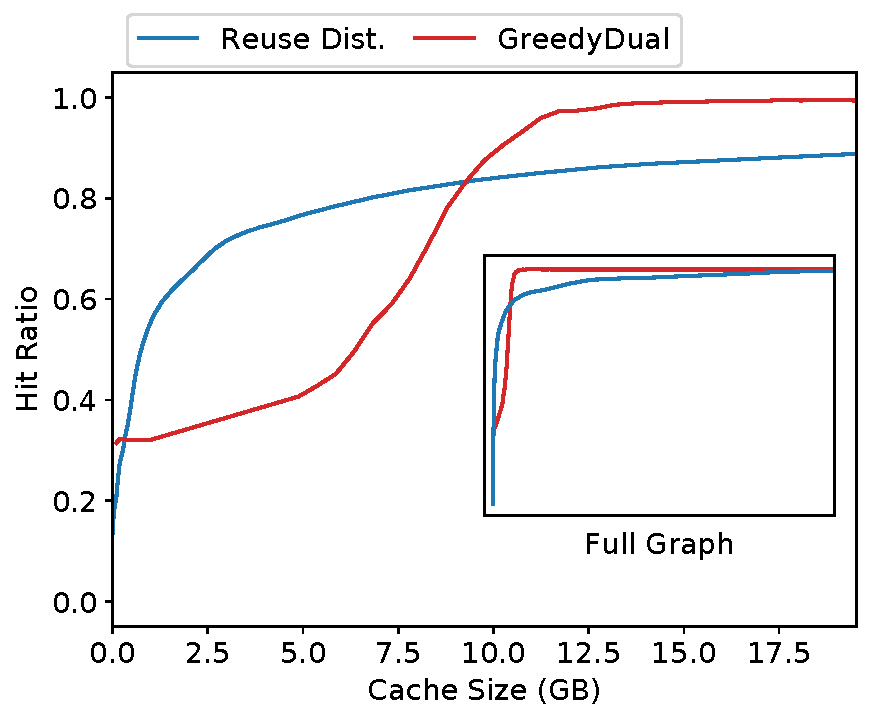
\includegraphics[width=0.3\textwidth]{../graphs/rep-funcs-392/hit-ratio-392-b.pdf}
  \caption{Hit ratio curve using reuse distances show slight deviations from the observed hit ratios due to dropped requests at lower sizes, and concurrent executions at higher sizes.}
  \label{fig:hrc}
\end{figure}

\paragraph{Limitations of the Caching Analogy.}
The error in hit-ratios with the reuse-distance approach in Figure~\ref{fig:hrc} highlights an important facet where caching does not fully map to FaaS.
The main difference is due to the limitations on the concurrent execution of functions. 
At lower cache sizes, a high miss rate results in higher server load, and hence a higher number of dropped requests, that the classical reuse-distance approaches do not capture.
If all warmed containers of a function are in use, then a new invocation results in a cold start---which would be counted as a cache ``hit''.
Thus at lower sizes, the real hit-ratio is lower than the ideal. 
At larger sizes, \emph{multiple} containers corresponding to concurrent invocations of a function will be present: which is again different from the caching model where objects are unique.
Reconciling these differences is an interesting area of future work.
However, we note that hit-ratio curves are only used for coarse-grained allocation.
Moreover, our dynamic allocation policy described next can fix these errors using proportional control. 


%\prat{Difference in two curves: could be because of multiple containers for a function, which is different from caching. So for larger cache sizes, the hit-ratio is higher. For lower sizes: it is lower because of dropped requests and not being able to handle the concurrent accesses which is not true with caching. So this is some sort of a negative result, or an area for future work.}


\subsection{Elastic Dynamic Scaling}
\label{subsec:dynamic}
\vspace*{\subsecspace}

We also use the hit-ratio curve approach for a \emph{dynamic} auto-scaling policy that adjusts the server size based on workload requirements. 
%
We assume that the FaaS server backend is running functions as containers either inside a virtual machine (VM), or is sharing the physical server with other cloud applications. 
In either case, it is important to be able to reclaim unused keep-alive cache resources and reduce its footprint, in order to increase the efficiency of the cloud platform. 

Our vertical elastic scaling policy is simple and is intended to demonstrate the efficacy of a general caching based approach. 
We implement a  proportional controller~\cite{pid-wiki} which periodically adjusts the VM memory size based on the rate of cold starts.  
Thus during periods of low rate of function invocations (i.e., arrival rate), the cache size can be reduced. 
This may \emph{increase} the miss-ratio---but we care about the cold starts (i.e., misses) per second, which is product of miss-ratio and invocations per second.
Our controller monitors the arrival and cold start rate, and uses the hit-ratio curve to decrease or increase VM size dynamically. 
We use VM resource deflation~\cite{deflation-eurosys19} to shrink or expand the VM by using a combination of hypervisor level page swapping, or guest-OS memory hot-plug and unplug. 


Assume that we have a target miss speed (number of cold starts/misses per second).
For instance, this target value can be a product of the desired hit-ratio, $h$, and the average function arrival rate for the entire workload trace, $\bar{\lambda}$. 
Periodically, we monitor the exponentially smoothed arrival rate $\lambda$, and the observed miss speed.
Our proportional controller adjusts the cache size in order to reduce the difference between the actual vs. target miss speed.
This error is used to compute the new \emph{miss rate}, $m$, and the associated cache size $c'$ as follows:
\begin{align}
  \label{eq:dyn}
%  m & = \frac{\bar{\lambda}}{\lambda}*h \\
  \text{HR}(c') & = 1-m = 1 - h\frac{\bar{\lambda}}{\lambda}
\end{align}

\noindent The new cache size $c'$ is then determined by inverting the hit-rate function $\text{HR}$.
Our vertical scaling controller is designed for coarse-grained VM size adjustments, and only tracks the workload at time granularities of several minutes. 
Our intent with this policy is to not be overly aggressive with the capacity changes, but only to capture the coarse diurnal effects. 
Therefore, we use a large error deadband: the cache size is only updated if the error is more than 30\%. 
%More sophisticated, predictive and reactive auto-scaling policies from web-clusters~\cite{gandhi2012autoscale} can be also be adapted. 
Finally, the memory scaling can also be combined with cpu auto-scaling based on the function arrival rate, using classical predictive and reactive auto-scaling techniques found in web-clusters~\cite{gandhi2012autoscale}. 




% Let the exponentially smoothed arrival rate of functions be $\lambda$. 

% The hit-ratio curve constructed for the static provisioning is applicable for the overall workload for the average arrival rate $\bar{\lambda}$.
% For the elastic scaling, we monitor the exponentially smoothed arrival rate, $EWMA(\lambda)$, and scale up or down if it is more than one standard deviation from $\bar{\lambda}$. 
% If $\lambda < \bar{\lambda}$, we scale the server's memory down by $\delta(m)$, which is determined based on the cache hit ratio curve to meet the average or the set number of misses per second. 


% Let current cache size be c, and load be $\lambda$.
% In general, the misses per second is given by $m = (1-HR(c))\lambda$.
% The goal is to keep this constant, that is $m = \bar{m}$.
% If the new cache size is $c'$, then we have: $(1-HR(c'))\lambda  = (1-HR(c))\bar{\lambda}$
% \begin{equation}
%   \label{eq:dyn} 
%   HR(c') = 1- \dfrac{(1-HR(c))\bar{\lambda}}{\lambda} 
% \end{equation}
% We use the hit-rate curve to thus find $c'$ that yields the hit-rate on the right hand side of the above equation.  

% tgt-miss-rate = avg-lambda/lambda*miss-ratio 


%%% Local Variables:
%%% mode: latex
%%% TeX-master: "paper"
%%% End:
